\begin{figure}[!htbp]
\centering
\subcaptionbox{Strong detonation}[0.45\textwidth]{
  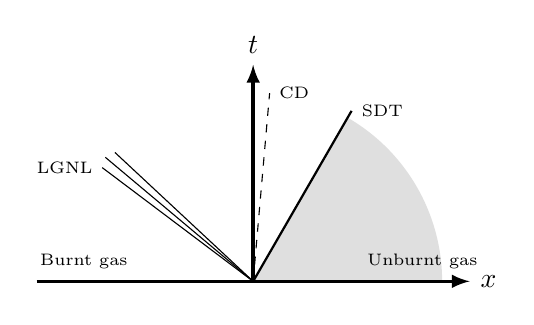
\begin{tikzpicture}[scale=.5]
    \tikzset{font={\fontsize{6pt}{10}\selectfont}}
    \fill [lightgray,opacity=.5] (0,0)--(4.8,0) arc(0:60:4.8);
    \draw[-latex,very thick](-5.5,0)--(5.5,0)
     node[right]{\normalsize $x$};
    \draw[-latex,very thick] (0,0)--(0,5.5)
  node[above] {\normalsize $t$};
    % \draw (2.7,0.3) node{$\bm U_r$};
    % \draw (-2.7,0.3) node{$\bm U_l$};
    % \draw (1.0,1.8) node{$\bm U_r^*$}; node[above]{\it $\bm{\mathcal W}_l$}
    % \draw (-1,1.5) node{$\bm U_l^*$}; node[above]{\it $\bm{\mathcal W}_r$}
    \draw [thick](0,0)--(60:5) node[right]{SDT};
    \draw (0,0)--(140:4.9);
    \draw (0,0)--(143:4.8) node[left]{LGNL};
    \draw (0,0)--(137:4.8);
    \draw[dashed] (0,0)--(85:4.8) node[right]{CD};
    \draw (4.3,0.5) node{Unburnt gas};
    \draw (-4.3,0.5) node{Burnt gas};
    \end{tikzpicture}
}
\hfil
\subcaptionbox{CJ detonation}[0.45\textwidth]{
  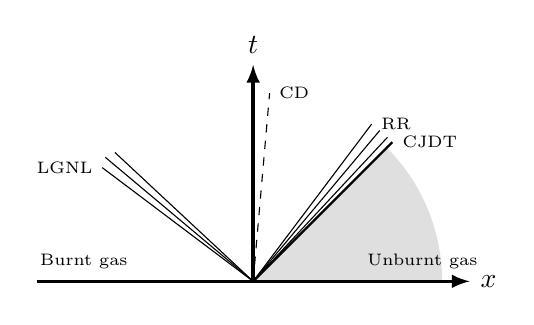
\begin{tikzpicture}[scale=.5]
    \tikzset{font={\fontsize{6pt}{10}\selectfont}}
    \fill [lightgray,opacity=.5] (0,0)--(4.8,0) arc(0:45:4.8);
    \draw[-latex,very thick](-5.5,0)--(5.5,0)
     node[right]{\normalsize $x$};
    \draw[-latex,very thick] (0,0)--(0,5.5)
  node[above] {\normalsize $t$};
    % \draw (2.7,0.3) node{$\bm U_r$};
    % \draw (-2.7,0.3) node{$\bm U_l$};
    % \draw (1.0,1.8) node{$\bm U_r^*$}; node[above]{\it $\bm{\mathcal W}_l$}
    % \draw (-1,1.5) node{$\bm U_l^*$}; node[above]{\it $\bm{\mathcal W}_r$}
    \draw [thick](0,0)--(45:5) node[right]{CJDT};
    \draw (0,0)--(47:5.0);
    \draw (0,0)--(50:5.0);
    \draw (0,0)--(53:5.0)node[right]{RR};
    \draw (0,0)--(140:4.9);
    \draw (0,0)--(143:4.8) node[left]{LGNL};
    \draw (0,0)--(137:4.8);
    \draw[dashed] (0,0)--(85:4.8) node[right]{CD};
    \draw (4.3,0.5) node{Unburnt gas};
    \draw (-4.3,0.5) node{Burnt gas};
    \end{tikzpicture}
}

\vspace{1em}

\subcaptionbox{Weak deflagration}[0.45\textwidth]{
  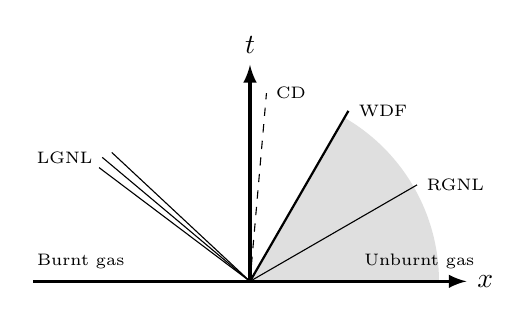
\begin{tikzpicture}[scale=.5]
  \tikzset{font={\fontsize{6pt}{10}\selectfont}}
  \fill [lightgray,opacity=.5] (0,0)--(4.8,0) arc(0:60:4.8);
  \draw[-latex,very thick](-5.5,0)--(5.5,0)
   node[right]{\normalsize $x$};
  \draw[-latex,very thick] (0,0)--(0,5.5)
node[above] {\normalsize $t$};
  % \draw (2.7,0.3) node{$\bm U_r$};
  % \draw (-2.7,0.3) node{$\bm U_l$};
  % \draw (1.0,1.8) node{$\bm U_r^*$}; node[above]{\it $\bm{\mathcal W}_l$}
  % \draw (-1,1.5) node{$\bm U_l^*$}; node[above]{\it $\bm{\mathcal W}_r$}
  \draw [thick](0,0)--(60:5) node[right]{WDF};
  \draw (0,0)--(30:4.9) node[right]{RGNL};
  \draw (0,0)--(140:4.9) node[left]{LGNL};
  \draw (0,0)--(143:4.8);
  \draw (0,0)--(137:4.8);
  \draw[dashed] (0,0)--(85:4.8) node[right]{CD};
  \draw (4.3,0.5) node{Unburnt gas};
  \draw (-4.3,0.5) node{Burnt gas};
  \end{tikzpicture}}
\hfil
\subcaptionbox{CJ deflagration}[0.45\textwidth]{
  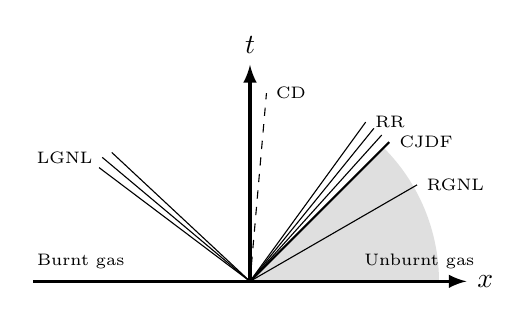
\begin{tikzpicture}[scale=.5]
   \tikzset{font={\fontsize{6pt}{10}\selectfont}}
    \fill [lightgray,opacity=.5] (0,0)--(4.8,0) arc(0:45:4.8);
    \draw[-latex,very thick](-5.5,0)--(5.5,0)
     node[right]{\normalsize $x$};
    \draw[-latex,very thick] (0,0)--(0,5.5)
  node[above] {\normalsize $t$};
    % \draw (2.7,0.3) node{$\bm U_r$};
    % \draw (-2.7,0.3) node{$\bm U_l$};
    % \draw (1.0,1.8) node{$\bm U_r^*$}; node[above]{\it $\bm{\mathcal W}_l$}
    % \draw (-1,1.5) node{$\bm U_l^*$}; node[above]{\it $\bm{\mathcal W}_r$}
    \draw [thick](0,0)--(45:5) node[right]{CJDF};
    \draw (0,0)--(30:4.9) node[right]{RGNL};
    \draw (0,0)--(48:5.0);
    \draw (0,0)--(51:5.0);
    \draw (0,0)--(54:5.0) node[right]{RR};
    \draw (0,0)--(140:4.9) node[left]{LGNL};
    \draw (0,0)--(143:4.8);
    \draw (0,0)--(137:4.8);
    \draw[dashed] (0,0)--(85:4.8) node[right]{CD};
    \draw (4.3,0.5) node{Unburnt gas};
    \draw (-4.3,0.5) node{Burnt gas};
    \end{tikzpicture}
}
  \caption{The Riemann problem for the reactive flow.
  LGNL: left non-linear wave; RGNL: right non-linear wave; CD: contact discontinuity; SDT: strong detonation; CJDT: CJ detonation; WDF: weak deflagration; CJDF: CJ deflagration; RR: right rarefaction wave.\label{fig:rp}}
\end{figure}